\chapter{Experiments}
\label{sec:experiments}

\section{Training setups}
\label{sec:training-setups}

\section{Graph-based models}
\label{Graph-based models}
\begin{figure}[]
    \centering
    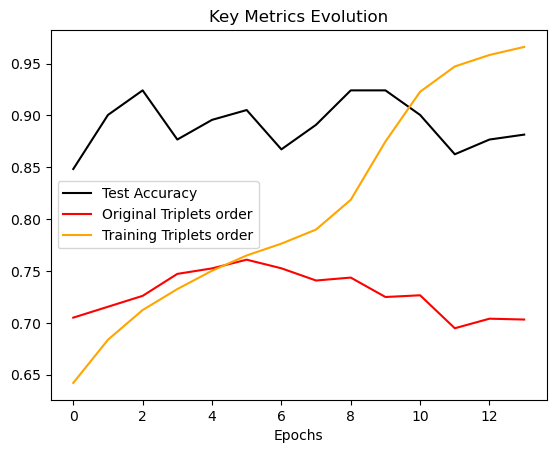
\includegraphics[width=0.5\columnwidth]{images/key_metrics_evolution_gnn.png}
    \caption{GNN model key metrics accuracies.}
    \label{fig:key_metrics_evolution_gnn}
\end{figure}

\begin{figure}[]
    \begin{subfigure}[h]{0.5\linewidth}
        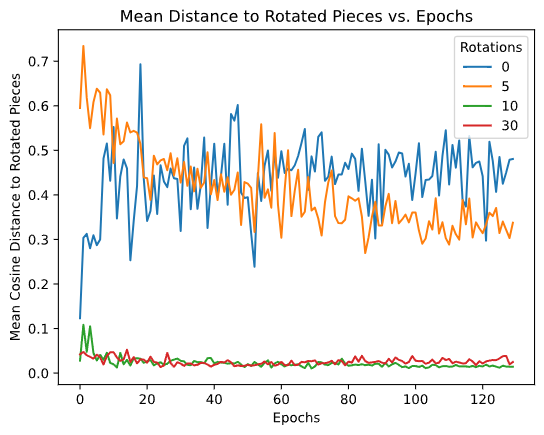
\includegraphics[width=\columnwidth]{images/mean_rotated_study.png}
        \caption{Mean distance to rotated distribution.}
        \label{fig:mean_rotated_study}
    \end{subfigure}
    \hfill
    \begin{subfigure}[h]{0.5\linewidth}
        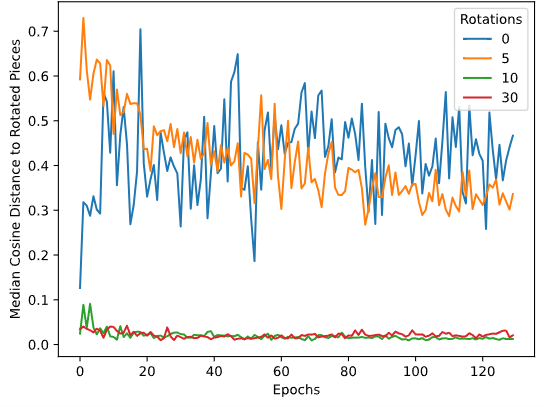
\includegraphics[width=\columnwidth]{images/median_rotated_study.png}
        \caption{Median distance to rotated distribution.}
        \label{fig:median_rotated_study}
    \end{subfigure}
    \caption{Influence of the number of rotations on the rotations metrics.}
\end{figure}

\begin{figure}[]
    \begin{subfigure}[h]{0.5\linewidth}
        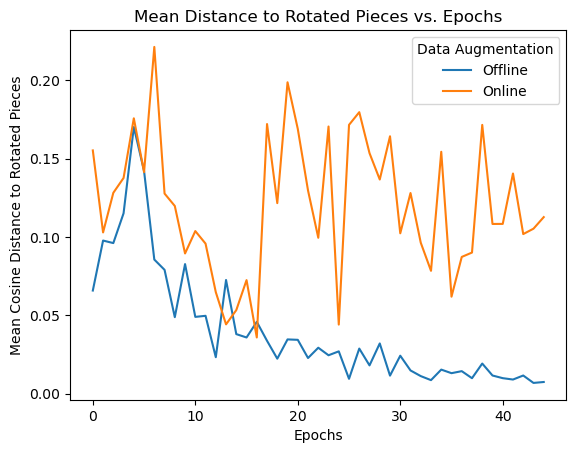
\includegraphics[width=\columnwidth]{images/mean_rotated_data_augmentation_type.png}
        \caption{Mean distance to rotated distribution.}
        \label{fig:mean_rotated_data_augmentation_type}
    \end{subfigure}
    \hfill
    \begin{subfigure}[h]{0.5\linewidth}
        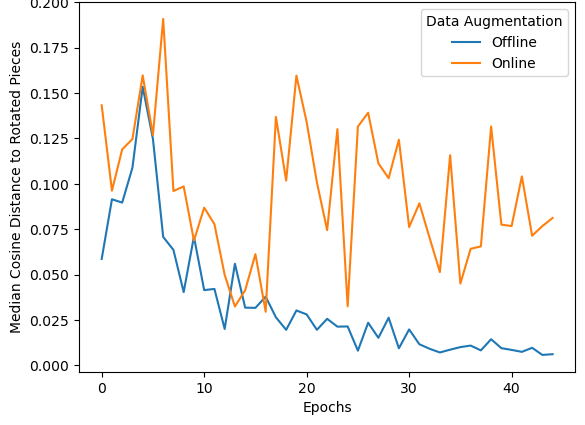
\includegraphics[width=\columnwidth]{images/median_rotated_data_augmentation_type.png}
        \caption{Median distance to rotated distribution.}
        \label{fig:median_rotated_data_augmentation_type}
    \end{subfigure}
    \caption{Influence of the type of data augmentation on the rotations metrics.}
\end{figure}

\section{Transformer-based models}
\label{Transformer-based models}

\begin{figure}[]
    \centering
    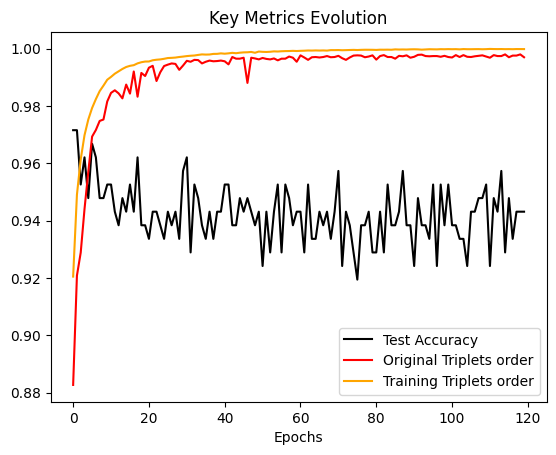
\includegraphics[width=0.5\columnwidth]{images/key_metrics_evolution_openshape.png}
    \caption{Fine-tuned model key metrics accuracies.}
    \label{fig:key_metrics_evolution_openshape}
\end{figure}

\begin{figure}[]
    \begin{subfigure}[h]{0.5\linewidth}
        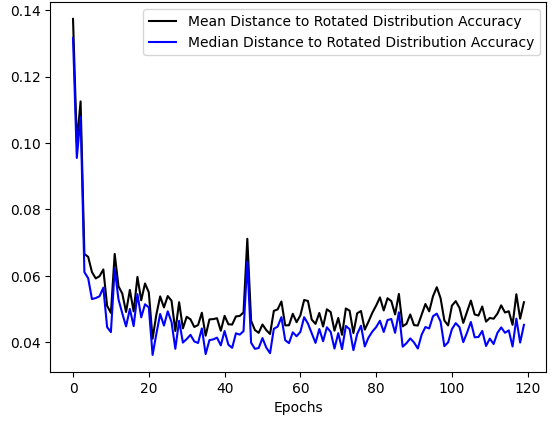
\includegraphics[width=\columnwidth]{images/rotation_metrics_evolution_openshape.png}
        \caption{Distances to rotated pieces accuracies.}
    \end{subfigure}
    \hfill
    \begin{subfigure}[h]{0.5\linewidth}
        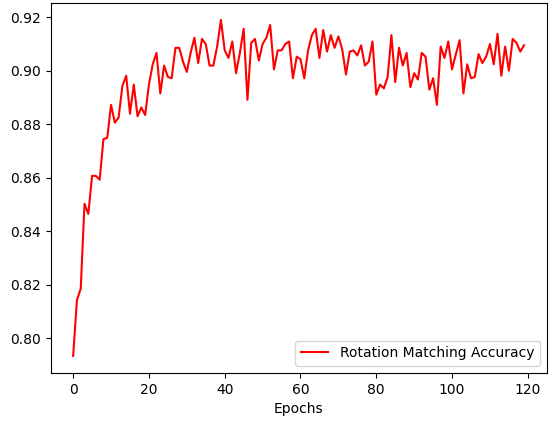
\includegraphics[width=\columnwidth]{images/rotation_accuracy_evolution_openshape.png}
        \caption{Rotation matching accuracy.}
    \end{subfigure}
    \caption{Fine-tuned model rotation accuracies.}
\end{figure}

%%% Local Variables: 
%%% mode: latex
%%% TeX-master: "isae-report-template"
%%% End: 